\documentclass[a4paper, 10pt]{article}

%% Mandatory stuff
\usepackage[utf8]{inputenc}
\usepackage[T1]{fontenc}
\usepackage[french]{babel}
%% --

\usepackage{amsmath}

%% Bitstream Charter for text and maths
%% with ye Olde french typography
%% Note: fake small caps
\usepackage[uppercase=upright,%
  greeklowercase=upright,%
  bitstream-charter]{mathdesign}
%% --

\usepackage{graphicx}

\title{Génération de labyrinthes avec des graphes}
\author{Yahya Kemal Karabulut\\Florent Marchand de Kerchove}

\begin{document}
%
\maketitle
%
%% Intro
%
Comment générer des labyrinthes intéressants à résoudre en utilisant
des graphes ? Nous présentons ici trois méthodes, dans un ordre de
difficulté des labyrinthes générés croissants, et de temps de
génération décroissant.

\subsection*{Définition du problème}

Nous voulons obtenir un labyrinthe comme on en trouve dans les pages
de jeux de certains magazines ; la figure \ref{fig:laby-canon} donne
un exemple d'un tel labyrinthe.

\begin{figure}[hbt]
  \centering
  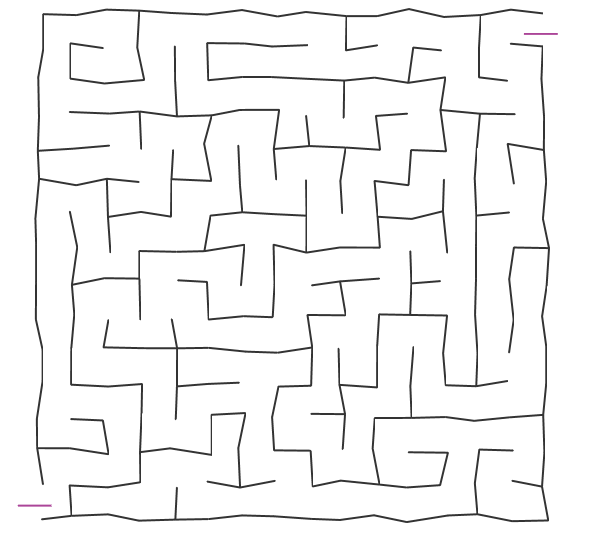
\includegraphics[height=5cm]{laby-canon.png}
  \caption{Labyrinthe idéal. En noir les murs, en rouge les deux
    issues. Le but est de relier les deux issues sans traverser les
    murs ni passer à l'extérieur.}
  \label{fig:laby-canon}
\end{figure}

Ces labyrinthes sont constitués de deux issues, typiquement placées à
l'opposé l'une de l'autre. L'une sera parfois appelée l'entrée, et
l'autre la sortie ; l'ordre n'a pas d'importance. Le but habituel, la
résolution du labyrinthe, est de trouver un chemin d'une issue à
l'autre en empruntant seulement les couloirs formés par les murs. Ce
qui nous intéresse ici, c'est de trouver une méthode pour générer un
tel labyrinthe d'une taille donnée, en utilisant des structures de
graphe. De préférence, cette méthode devra donner des labyrinthes
légèrement difficiles à résoudre.

%% Méthode 1
\subsection*{Retrait aléatoire de murs}

On peut rapidement élaborer une première méthode en partant d'un
graphe isomorphe à une grille de côté $n$, et en lui ôtant des arêtes
(les murs) jusqu'à l'apparition d'un chemin entre les deux issues.

Le graphe est facile à créer~: $n * n$ sommets sont disposés en
grille, et des arêtes relient chaque sommet à ses voisins (entre deux
et quatre). Ensuite, on place les deux issues, ce qui revient à ôter
deux murs extérieurs ; on peut les choisir aléatoirement, mais autant
les prendre à des coins opposés de la grille pour maximiser la
distance à parcourir. Retirer des arêtes choisies aléatoirement est
simple, il faut juste faire attention à ne pas retirer des arêtes du
bord du labyrinthe, puisque l'extérieur du labyrinthe n'est pas un
couloir acceptable. Enfin, pour déterminer si un chemin existe entre
les deux issues, il suffit de conserver le mur d'une des deux issues
dans le graphe, et remarquer que pour qu'un chemin solution existe, ce
mur doit être un isthme ; c'est à dire que s'il est enlevé, le graphe
gagne une composante connexe.

Le principe n'est pas compliqué, et le résultat escompté est
obtenu. En revanche, il n'est pas très convaincant car les couloirs
sont larges, ce qui facilite grandement la résolution du labyrinthe,
et le temps de calcul n'est pas idéal non plus. On peut complexifier
les labyrinthes en refusant de retirer des arêtes qui ont un degré
trop bas, mais il y a un degré minimal requis pour s'assurer qu'un
isthme soit possible (fig. \ref{fig:laby-isthm}).

\begin{figure}[hbt]
  \centering
  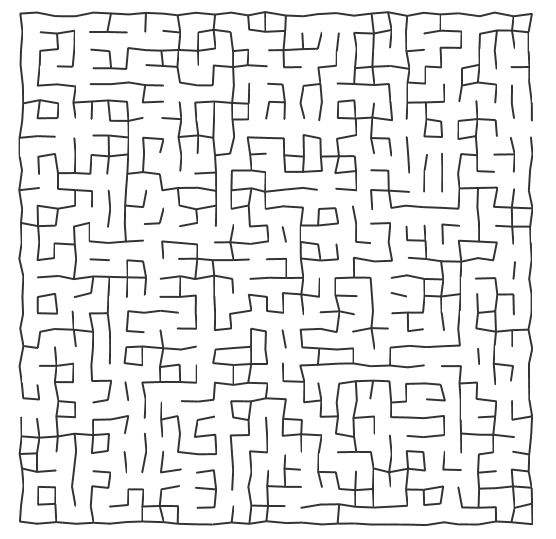
\includegraphics[height=7cm]{laby-isthm.png}
  \caption{Labyrinthe obtenu avec le retrait aléatoire de murs, en
    refusant de retirer les murs ayant un degré trop bas. Il y
    beaucoup de couloirs inaccessibles et le chemin est facile à
    trouver.}
  \label{fig:laby-isthm}
\end{figure}

%% Méthode 2
\subsection*{Arbre couvrant de poids minimal}

La seconde méthode repose sur le graphe «~négatif~» du précédent~:
celui formé par les couloirs du labyrinthe. Dans ce graphe, les
sommets sont des pièces, et la présence d'une arête reliant deux
pièces signifie qu'un passage est possible entre les deux. Cette
notion de passage est naturellement adaptée aux modèles par des
graphes, ce qui va nous permettre d'utiliser des méthodes classiques.

Dans ce modèle, pour qu'un chemin existe entre les deux issues, il
faut simplement qu'un chemin existe sur le graphe entre les deux
sommets qui les représentent. Dans l'état de départ où il existe une
arête d'une pièce à toutes ses voisines, c'est bien sûr le cas, mais
cela correspond à l'absence totale de murs interne ; ça donne un
labyrinthe sans intérêt. Il faut restreindre le nombre de chemins
possibles entre les deux issues. Justement, il y a des graphes
particuliers qui assurent l'existence d'un chemin unique entre toute
paire de leurs sommets~: les arbres. Il nous suffit donc de
transformer notre graphe en arbre, et même en arbre couvrant pour
s'assurer de passer par tous ses sommets.

\begin{figure}[hbt]
  \centering
  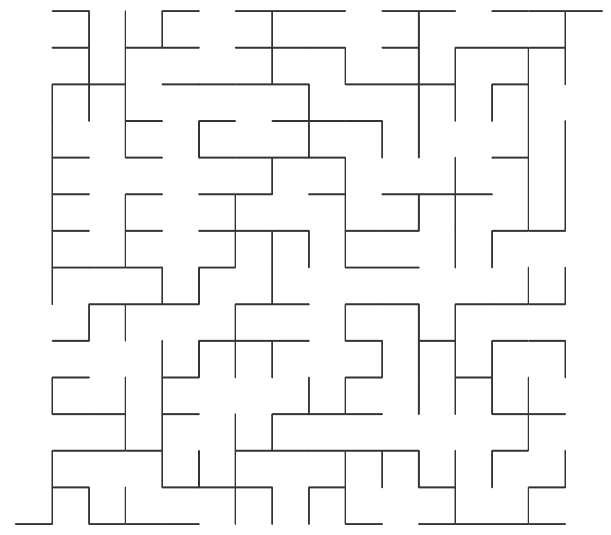
\includegraphics[height=4cm]{laby-tree.png}
  \caption{Arbre couvrant des couloirs d'un labyrinthe. Toutes les
    pièces sont accessibles.}
  \label{fig:laby-tree}
\end{figure}

Nous devons d'abord construire le graphe qui contient tous les
couloirs~: c'est une grille, comme dans la première méthode. Ensuite,
il faut ne garder qu'un arbre couvrant de ce graphe. Pour ce faire, on
peut utiliser l'algorithme de Prim (ou de Kruskal), en attribuant des
poids aléatoires à chaque arête afin de varier le labyrinthe. Mais
avoir cet arbre (fig. \ref{fig:laby-tree}) ne nous donne pas notre
labyrinthe, car il faut reconvertir ce modèle en son «~négatif~»~:
c'est à dire placer des murs tout autour des pièces, là où il n'y a
pas de couloirs, ainsi que les murs extérieurs.

\begin{figure}[hbt]
  \centering
  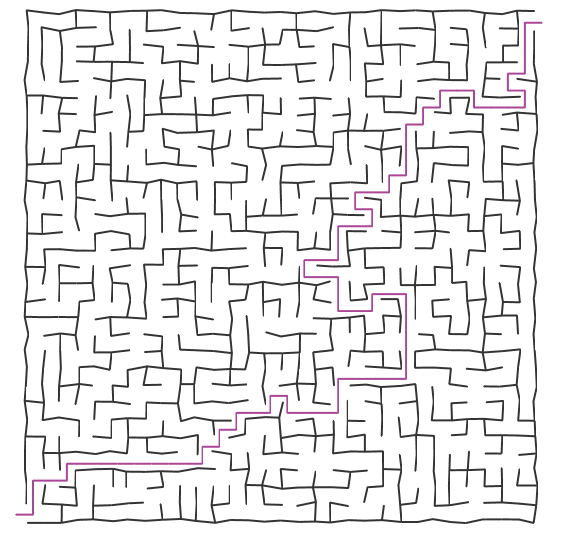
\includegraphics[height=7cm]{laby-prim.png}
  \caption{Labyrinthe obtenu à partir d'un arbre couvrant. Il n'y a
    plus de couloirs inaccessible, mais le chemin reste facile à
    trouver.}
  \label{fig:laby-prim}
\end{figure}

Les labyrinthes obtenus par cette méthode (fig. \ref{fig:laby-prim}
pour un exemple) n'ont plus aucun trou ni couloir inaccessible,
contrairement à ceux de la méthode précédente. C'est un très bon
point. De plus, la terminaison de l'algorithme est plus prévisible,
même si le calcul d'arbre couvrant n'a pas une complexité légère. En
revanche, l'attribution aléatoire de poids aux arêtes donne des
solutions prévisibles qui ont tendance à épouser la ligne droite, et
les culs-de-sac ne sont pas suffisamment profond pour s'y
perdre. C'est évidemment inacceptable pour tout amateur de labyrinthe
qui se respecte ; même un minotaure n'en voudrait pas. Nous pouvons
jouer sur la distribution aléatoire des poids des arêtes afin de
donner une forme voulue à la solution, mais la méthode suivante résout
le problème plus simplement.

%% Méthode 3
\subsection*{Marche en profondeur}

Plutôt que de créer un arbre couvrant de poids minimal en utilisant
une distribution de poids aléatoire, nous allons simplement créer un
arbre couvrant quelconque. Deux méthodes classiques s'offrent à nous~:
le parcours en largeur, et celui en profondeur. En vertu de sa
définition, le premier va créer des labyrinthes aux couloirs
rectilignes, donc ennuyeux. En revanche, le second va nous donner les
chemins tortueux convoités, précisément parce qu'il élabore l'arbre en
profondeur.

Nous apportons donc une légère modification à la méthode précédente~:
la création de l'arbre n'utilise plus l'algorithme de Prim, mais un
algorithme de parcours en profondeur qui choisit ses arêtes non
visitées dans un ordre aléatoire.

\begin{figure}[hbt]
  \centering
  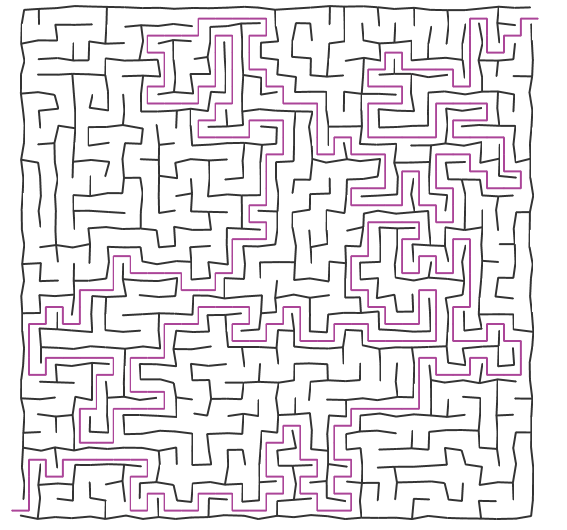
\includegraphics[height=7cm]{laby-depth.png}
  \caption{Labyrinthe à la solution particulièrement tortueuse typique
    de la marche en profondeur.}
  \label{fig:laby-depth}
\end{figure}

La figure \ref{fig:laby-depth} atteste de la difficulté des
labyrinthes obtenus par cette méthode. Qui plus est, nous sommes
passés de l'algorithme de Prim à une marche en profondeur résolument
plus rapide. Cette méthode n'a donc que des avantages sur les
précédentes.

\subsection*{Améliorations}

Nous nous sommes arrêtés à la troisième méthode qui donne des
labyrinthes suffisamment intéressants selon les critères que nous nous
étions fixés au début, mais il pourrait être souhaitable d'avoir un
contrôle plus fin sur le chemin qui relie les deux issues. À
l'extrême, on pourrait envisager spécifier complètement ce chemin, et
un algorithme viendrait le compléter en arbre couvrant, en utilisant
par exemple la marche en profondeur.

Pour introduire un peu de variété, on pourrait également adapter la
dernière méthode pour produire des graphes aux formes moins familières
que la grille : losanges, ellipses, spirales, \dots. Les
transformations linéaires peuvent facilement s'effectuer, les autres
sont moins évidentes. C'est d'ailleurs par le labyrinthe légèrement
exotique qui suit que nous terminerons.

\vfill

\begin{center}
\makebox[\linewidth]{
  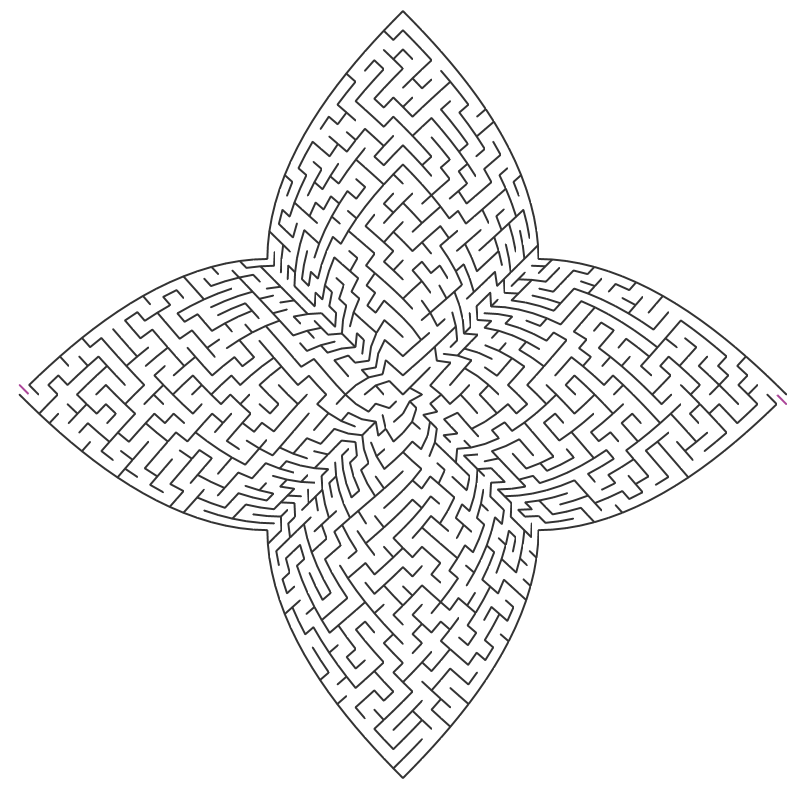
\includegraphics[height=15cm]{laby-hell.png}
}
\end{center}

%
\end{document}
